% tikzpic.tex
\documentclass[crop,tikz]{standalone}% 'crop' is the default for v1.0, before it was 'preview'

\usetikzlibrary{arrows,decorations.pathmorphing,decorations.pathreplacing,backgrounds,positioning,fit,matrix}
\usetikzlibrary{shapes,calc,patterns,arrows.meta}
\tikzset{
	vert/.style={circle,inner sep=1.5,fill=white,draw,minimum size=.3cm},
	edge/.style={color=black, thick},
	diredge/.style={->,>={Stealth[width=8pt,length=8pt]},color=black, thick},
	timelabel/.style={fill=white,font=\footnotesize, text centered},
	wave/.style={decorate,decoration={coil,aspect=0}},
	dirwave/.style={->, >={Stealth[width=8pt,length=8pt]},decorate,decoration={coil,aspect=0}},
	diredge2/.style={->,>={Stealth[width=8pt,length=8pt]}}
}
\begin{document}
	
	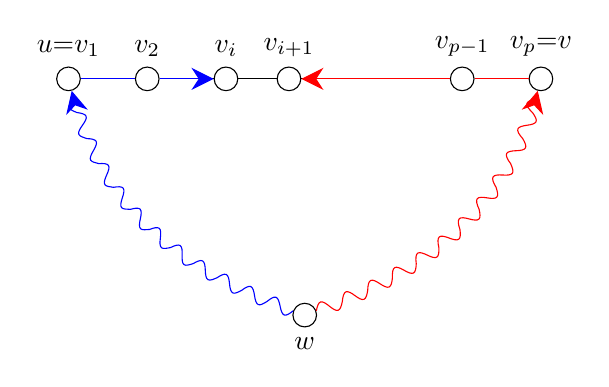
\begin{tikzpicture}
		%%%S_uv
		\node[vert,label=above:$u {=} v_1$] (v1) at (1,0) {};
		\node[vert,label=above:$v_2$] (v2) at (2,0) {};
		\node[vert,label=above:$v_i$] (vi) at (3,0) {};
		\node[vert,label=above:$v_{i+1}$] (vi+1) at (3.8,0) {};
		\node[vert,label=above:$v_{p-1}$] (vp1) at (6,0) {};
		\node[vert,label=above:$v_p {=} v$] (vp) at (7,0) {};
		\draw (v1) -- (v2) -- (vi) -- (vi+1) -- (vp1) -- (vp);
		
		%%%% node w
		\node[vert,label=below:$w$] (w) at (4,-3) {};
		
		
		
		\draw [blue] 
		(w) edge[dirwave] [out=160,in=285] (v1) 
		(v1) -- (v2)
		(v2) edge[diredge2] (vi);
		
		\draw [red]
		(w) edge[dirwave] [out=20,in=255] (vp) 
		(vp) -- (vp1)
		(vp1) edge[diredge2] (vi+1);
		
	\end{tikzpicture}
	
	
\end{document}